\chapter {Introduction}

\section{Why do we try to predict seasonal influenza evolution?}

Seasonal influenza infects 5--15\% of the global population yearly causing 100,000s of deaths and influenza subtype A/H3N2 is responsible for the bulk of human mortality and morbidity \citep{WHO2009}.
Influenza virus naturally evolves to escape acquired immunity in the human population and this evolution results in loss of vaccine efficacy over time as the virus evolves away from the chosen vaccine strain.
This process of \textit{antigenic drift} necessitates yearly selection of vaccine strains by the World Health Organization (WHO).
Manufacture and distribution of the influenza vaccine takes almost one year and the vaccine can contain only one representative strain per seasonal influenza subtype (A/H3N2, A/H1N1pdm, B/Victoria, and B/Yamagata).
As a result, WHO officials must predict which currently circulating A/H3N2 strain will be more representative of the influenza population one year in the future.
The predictions required for vaccine development have been historically challenging, but recent improvements in sequencing throughput and developments in computational models have made the prediction of influenza virus evolution more tractable \citep{Lassig:2017hr,Morris:2017ea}.
The better these predictions are, the more likely the vaccine will prevent illness and death from infection.

\section{How do we think seasonal influenza evolves?}

Globally successful seasonal influenza viruses are usually antigenically distinct from previous lineages \citep{Smith:2004jc}.
Thus, antigenic drift is an important predictor for influenza surveillance and vaccine recommendations \citep{Morris:2017ea}.
Antigenic drift occurs through mutations to the hemagglutinin (HA) surface protein that abrogate binding of preexisting human antibodies.
Antigenic phenotype is most commonly measured through the hemagglutination inhibition (HI) assay, which quantifies the extent to which antisera blocks attachment of viruses to red blood cells \citep{hirst1943studies}.
HI assays are the gold standard for measuring antigenic drift phenotypes, but these experiments are typically low-throughput and laborious compared to modern genome sequencing \citep{Wood:2012ii}.
Thus, researchers have attempted to predict viral success by estimating antigenic drift from HA genome sequences alone \citep{Luksza:2014hj,Steinbruck:2014kq,Neher:2014eu}.

Seasonal influenza viruses rapidly accumulate mutations during replication, due to their error-prone RNA polymerase.
For most genes, most new amino acid mutations will weaken the functionality of their corresponding proteins and reduce viral fitness.
An exception to this rule are amino acid mutations in HA or the other primary surface protein, neuraminidase (NA), that modify binding sites of host antibodies from previous viral exposure.
These mutations contribute to antigenic drift and increase viral fitness by allowing viruses to escape existing antibodies (Figure~\ref{fig:beneficial-and-deleterious-mutations-in-ha}).
Thus, mutations in HA and NA create fitness trade-offs, where beneficial mutations facilitate antigenic drift against a background of deleterious mutations.

\begin{figure}
  \centering
  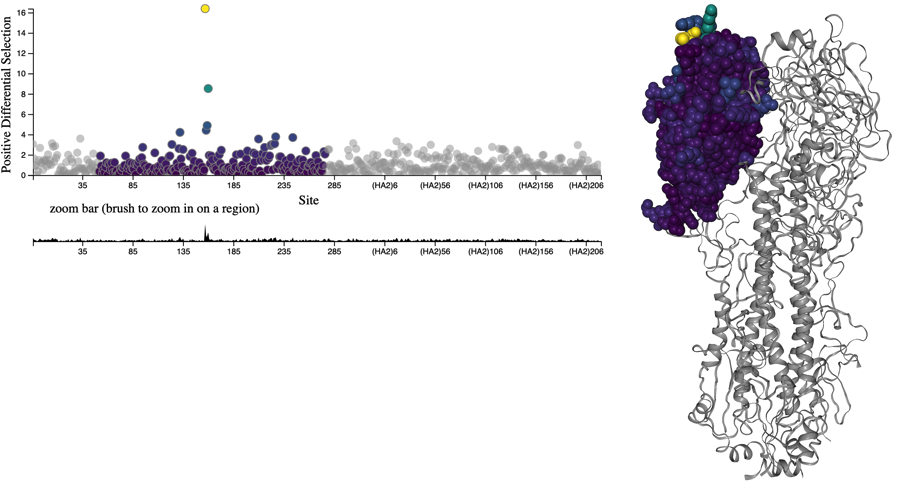
\includegraphics[width=\columnwidth]{chapter_05/flu-forecasting-beneficial-and-deleterious-mutations-in-ha.png}
  \caption{HA accumulates beneficial mutations in its head domain (sites with color) that enable escape from antibody binding and deleterious mutations in its stalk domain (sites in gray) that reduce its ability to infect new host cells.
    The linear genome view on the left shows how sites from HA's head domain map to the three-dimensional structure of an HA trimer.
    The site highlighted in yellow reveals where different amino acid mutations allowed a seasonal influenza virus to escape binding from existing antibodies in a human's polyclonal sera \citep{Lee2019}.
    \href{https://dms-view.github.io/?markdown-url=https\%3A\%2F\%2Fdms-view.github.io\%2Fdata\%2FIAV\%2Flee2019mapping.md&data-url=https\%3A\%2F\%2Fdms-view.github.io\%2Fdata\%2FIAV\%2Fflu_dms-view.csv&condition=2009-age-53&site_metric=site-Positive+Differential+Selection&mutation_metric=mut-Positive+Differential+Selection&selected_sites=52\%2C53\%2C54\%2C55\%2C56\%2C57\%2C58\%2C59\%2C60\%2C61\%2C62\%2C63\%2C64\%2C65\%2C66\%2C67\%2C68\%2C69\%2C70\%2C71\%2C72\%2C73\%2C74\%2C75\%2C76\%2C77\%2C78\%2C79\%2C80\%2C81\%2C82\%2C83\%2C84\%2C85\%2C86\%2C87\%2C88\%2C89\%2C90\%2C91\%2C92\%2C93\%2C94\%2C95\%2C96\%2C97\%2C98\%2C99\%2C100\%2C101\%2C102\%2C103\%2C104\%2C105\%2C106\%2C107\%2C108\%2C109\%2C110\%2C111\%2C112\%2C113\%2C114\%2C115\%2C116\%2C117\%2C118\%2C119\%2C120\%2C121\%2C122\%2C123\%2C124\%2C125\%2C126\%2C127\%2C128\%2C129\%2C130\%2C131\%2C132\%2C133\%2C134\%2C135\%2C136\%2C137\%2C138\%2C139\%2C140\%2C141\%2C142\%2C143\%2C144\%2C145\%2C146\%2C147\%2C148\%2C149\%2C150\%2C151\%2C152\%2C153\%2C154\%2C155\%2C156\%2C157\%2C158\%2C159\%2C160\%2C161\%2C162\%2C163\%2C164\%2C165\%2C166\%2C167\%2C168\%2C169\%2C170\%2C171\%2C172\%2C173\%2C174\%2C175\%2C176\%2C177\%2C178\%2C179\%2C180\%2C181\%2C182\%2C183\%2C184\%2C185\%2C186\%2C187\%2C188\%2C189\%2C190\%2C191\%2C192\%2C193\%2C194\%2C195\%2C196\%2C197\%2C198\%2C199\%2C200\%2C201\%2C202\%2C203\%2C204\%2C205\%2C206\%2C207\%2C208\%2C209\%2C210\%2C211\%2C212\%2C213\%2C214\%2C215\%2C216\%2C217\%2C218\%2C219\%2C220\%2C221\%2C222\%2C223\%2C224\%2C225\%2C226\%2C227\%2C228\%2C229\%2C230\%2C231\%2C232\%2C233\%2C234\%2C235\%2C236\%2C237\%2C238\%2C239\%2C240\%2C241\%2C242\%2C243\%2C244\%2C245\%2C246\%2C247\%2C248\%2C249\%2C250\%2C251\%2C252\%2C253\%2C254\%2C255\%2C256\%2C257\%2C258\%2C259\%2C260\%2C261\%2C262\%2C263\%2C264\%2C265\%2C266\%2C267\%2C268\%2C269\%2C270\%2C271\%2C272\%2C273\%2C274\%2C275\%2C276&protein-data-color=&protein-other-color=&pdb-url=https\%3A\%2F\%2Fdms-view.github.io\%2Fdata\%2FIAV\%2F4O5N_trimer.pdb}{Explore this figure interactively with dms-view}.\label{fig:beneficial-and-deleterious-mutations-in-ha}
  }
\end{figure}

Viruses carrying beneficial mutations should grow exponentially relative to viruses lacking those mutations (Figure~\ref{fig:exponential-growth-with-clonal-interference}A).
Beneficial mutations on different genetic backgrounds will compete with each other in a process known as clonal interference (Figure~\ref{fig:exponential-growth-with-clonal-interference}B).
If beneficial mutations have large effects on fitness, the fitness of the genetic background where the beneficial mutations occur is less important for the success of the virus than the fitness effect of the beneficial mutations themselves (Figure~\ref{fig:fitness-landscape-by-mutation-effect-size}).
If beneficial mutations have similar, smaller effects on fitness, a virus's overall fitness depends on the effect of the beneficial mutations and the relative fitness of its genetic background.
In this case, the ultimate success and fixation of these beneficial mutations depends, in part, on the number of deleterious mutations that already exist in the same genome (Figure~\ref{fig:fixation-probability-as-function-of-background}).

\begin{figure}
  \centering
  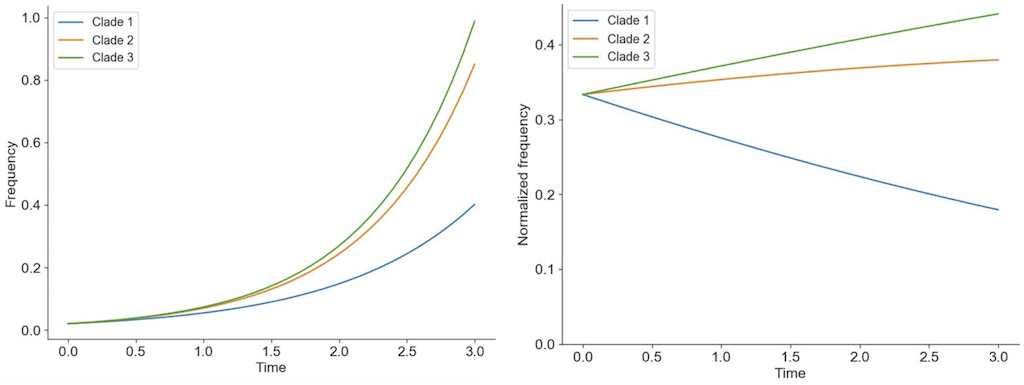
\includegraphics[width=\columnwidth]{chapter_05/flu-forecasting-exponential-growth-with-clonal-interference.png}
  \caption{Individuals in asexually reproducing populations tend to grow exponentially relative to their fitness (left).
    Normalization of frequencies to sum to 100\% represents competition between viruses for hosts through clonal interference and reveals how exponentially growing viruses can decrease in frequency when their relative fitness is low (right).\label{fig:exponential-growth-with-clonal-interference} }
\end{figure}

\begin{figure}
  \centering
  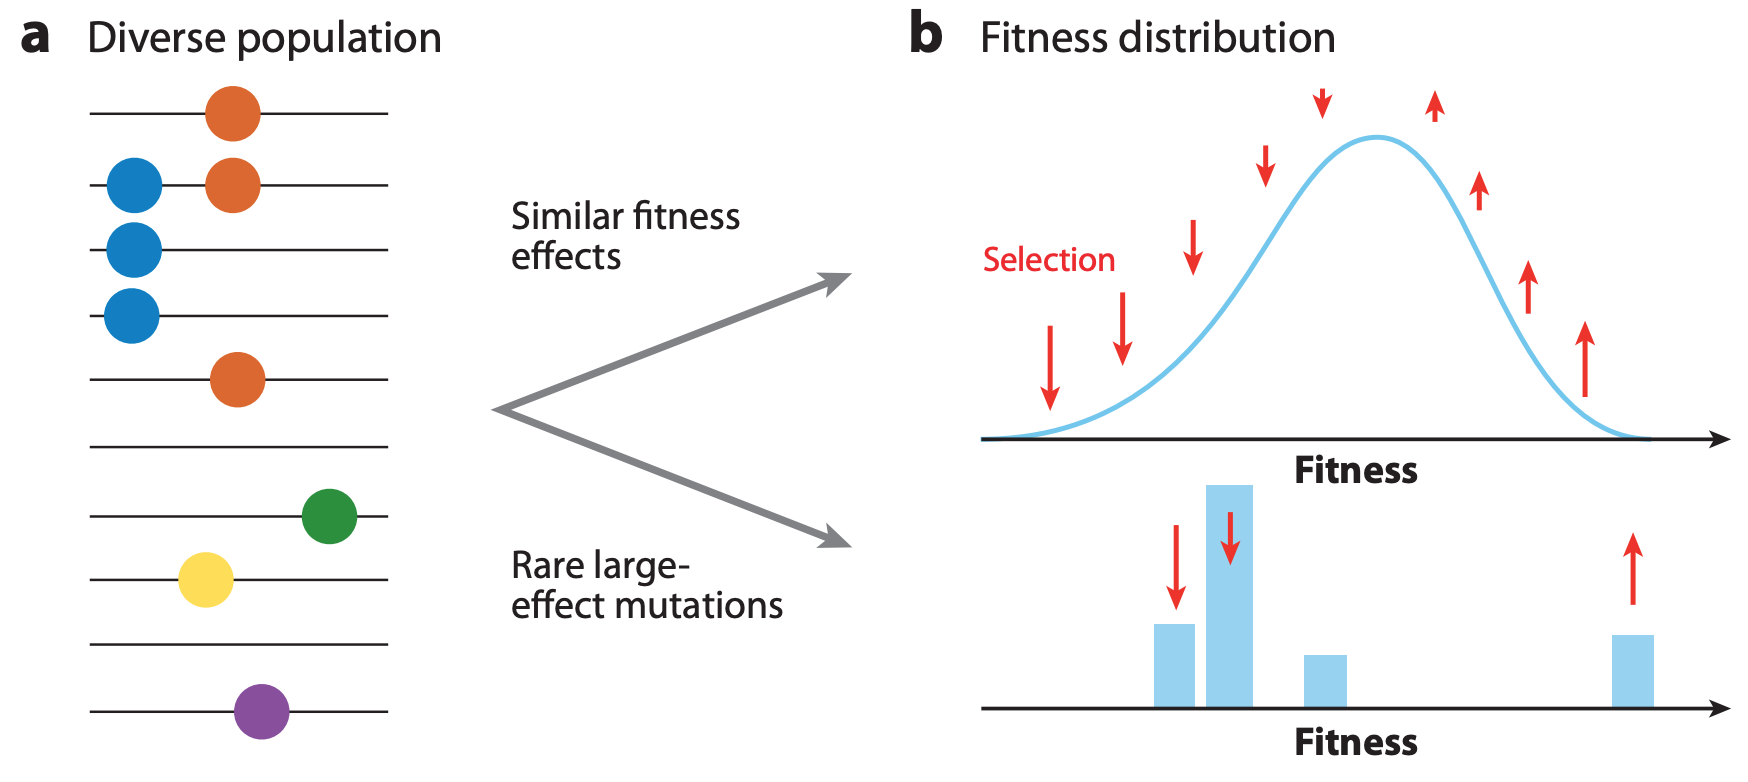
\includegraphics[width=\columnwidth]{chapter_05/flu-forecasting-fitness-landscape-by-mutation-effect-size.png}
  \caption{The shape of fitness landscapes depends, in part, on mutation effect sizes.
    Mutations with similar, smaller effects (blue and orange circles) produce a smooth Gaussian fitness distribution while mutations with large effect sizes (green, yellow, and purple circles) produce a more discrete fitness distribution.
    From Figure 1A and B of \citet{Neher2013}.\label{fig:fitness-landscape-by-mutation-effect-size} }
\end{figure}

\begin{figure}
  \centering
  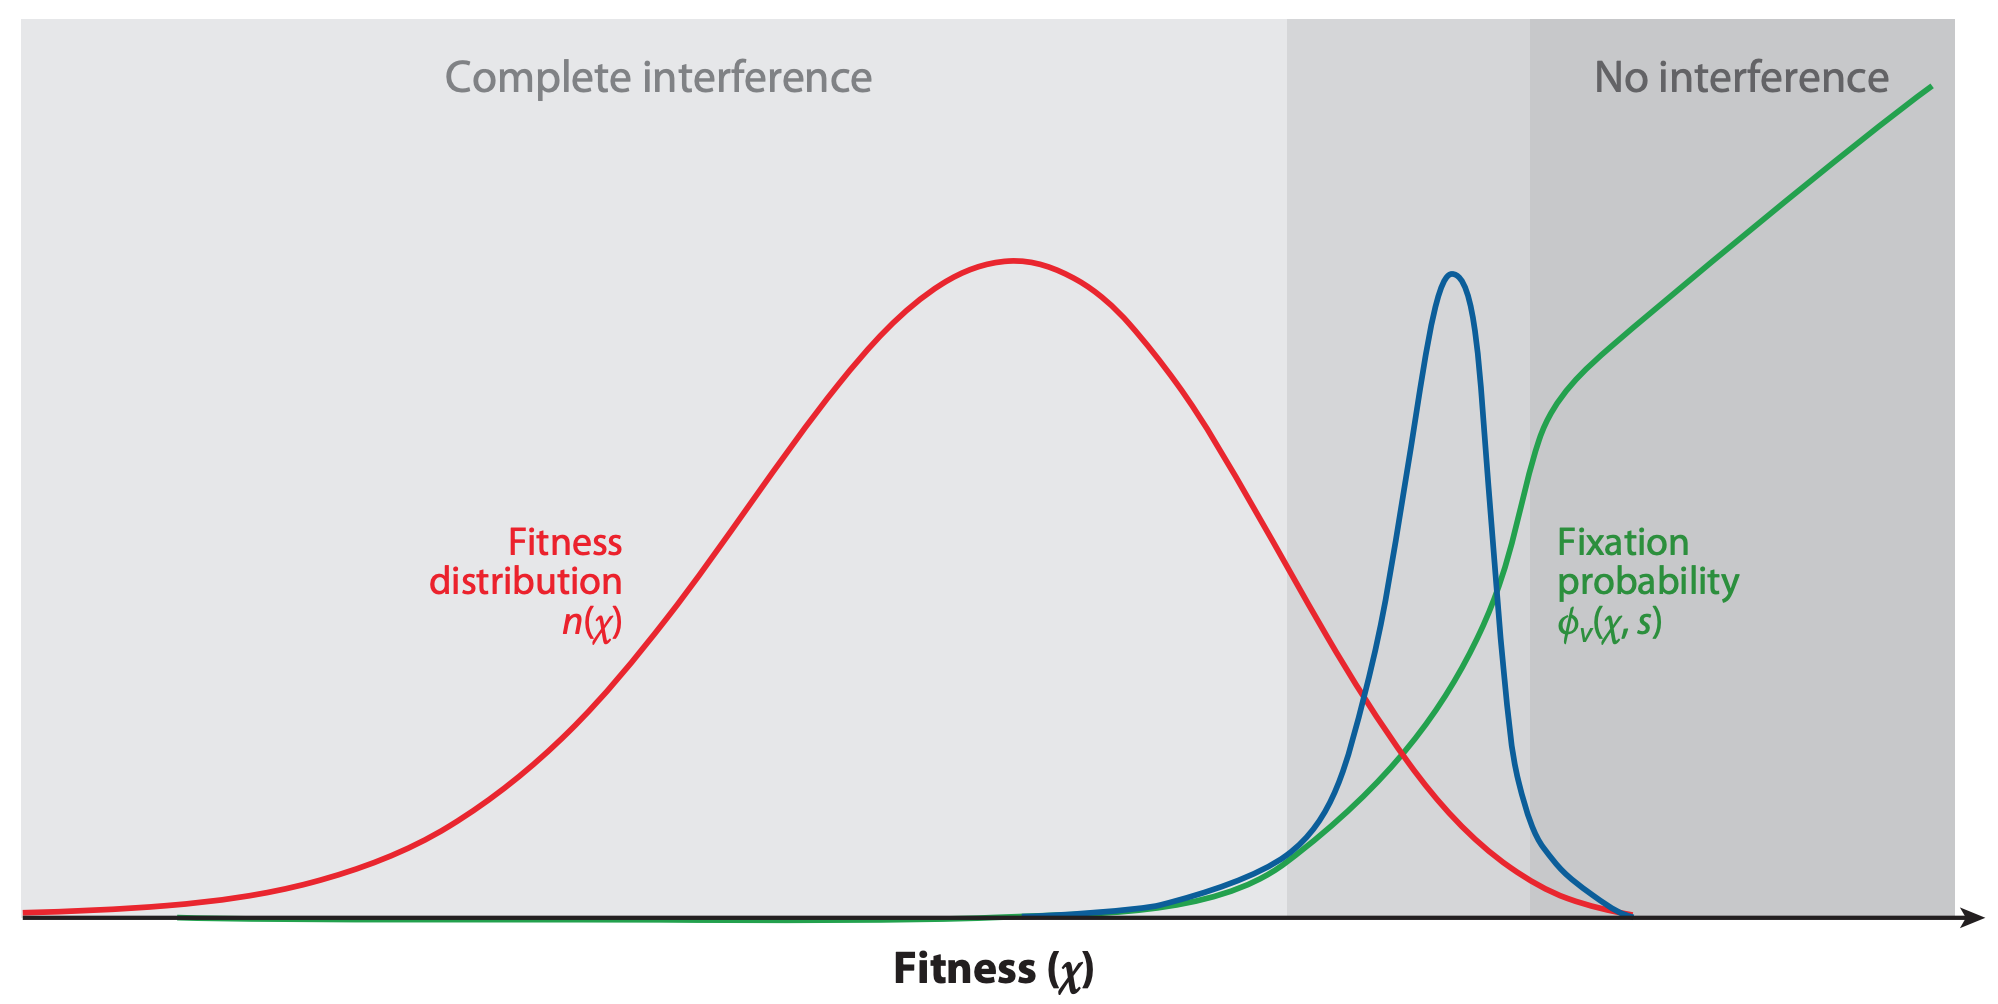
\includegraphics[width=\columnwidth]{chapter_05/flu-forecasting-fixation-probability-as-function-of-background.png}
  \caption{The fixation probability of a beneficial mutation is a function of the mutation's genetic background.
    When mutations have similar, smaller effects, the fitness of a beneficial mutation's genetic background (red) contributes to the mutation's fixation probability (green).
    Mutations that ultimately fix originate from distribution given by the product of the background fitness and the fixation probability (blue).
    From Figure 2C of \citet{Neher2013}.\label{fig:fixation-probability-as-function-of-background} }
\end{figure}

\section{What is predictable about seasonal influenza evolution?}

The expectations from population genetic theory described above and previous experimental work suggest that aspects of seasonal influenza's evolution might be predictable.
Mutations in HA and NA that alter host antibody binding sites and enable viruses to reinfect hosts should be under strong positive selection.
We expect these strongly beneficial mutations to sweep through the global seasonal influenza population at a rate that depends on the importance of their genetic background.
We also do not expect that every site in HA or NA will acquire beneficial mutations.
For example, fewer than a quarter of HA's 566 amino acid sites are under positive selection \citep{Bush:1999vj}, have undergone rapid sweeps \citep{Shih:2007bd}, or contributed to antigenic drift \citep{Wolf:2006da}.
Importantly, not all of these sites contribute equally to antigenic drift \citep{Koel:2013jz}.
Additionally, the complex and strong pressures of existing human immunity appear to constrain the space of antigenic phenotypes that viruses can explore at any given time \citep{Smith:2004jc,Bedford2012}.

Recently, researchers have built on this evidence to create formal predictive models of seasonal influenza evolution.
\citet{Neher:2014eu} used expectations from traveling wave models to define the ``local branching index'' (LBI), an estimate of viral fitness.
LBI assumes that most extant viruses descend from a highly fit ancestor in the recent past and uses patterns of rapid branching in phylogenies to identify putative fit ancestors (Figure~\ref{fig:lbi}).
\citet{Neher:2014eu} showed that LBI could successfully identify individual ancestral nodes that were highly representative of the seasonal influenza population one year in the future.

\begin{figure}
  \centering
  \begin{subfigure}[b]{0.5\columnwidth}
    \centering
    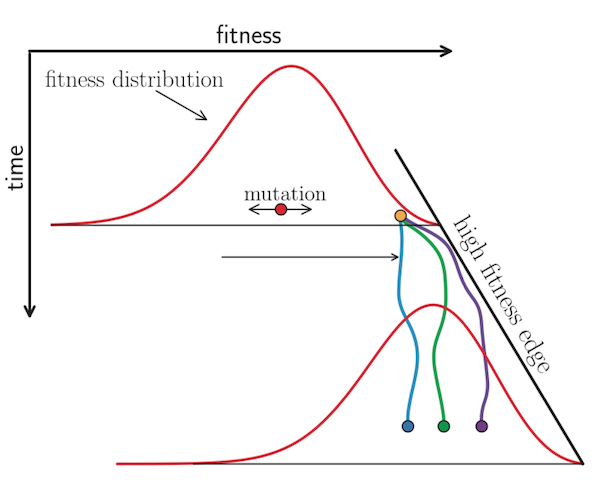
\includegraphics[width=\textwidth]{chapter_05/flu-forecasting-neher-2013-figure-5d.png}
    \label{fig:lbi-theory}
  \end{subfigure}

  \begin{subfigure}[b]{0.65\columnwidth}
    \centering
    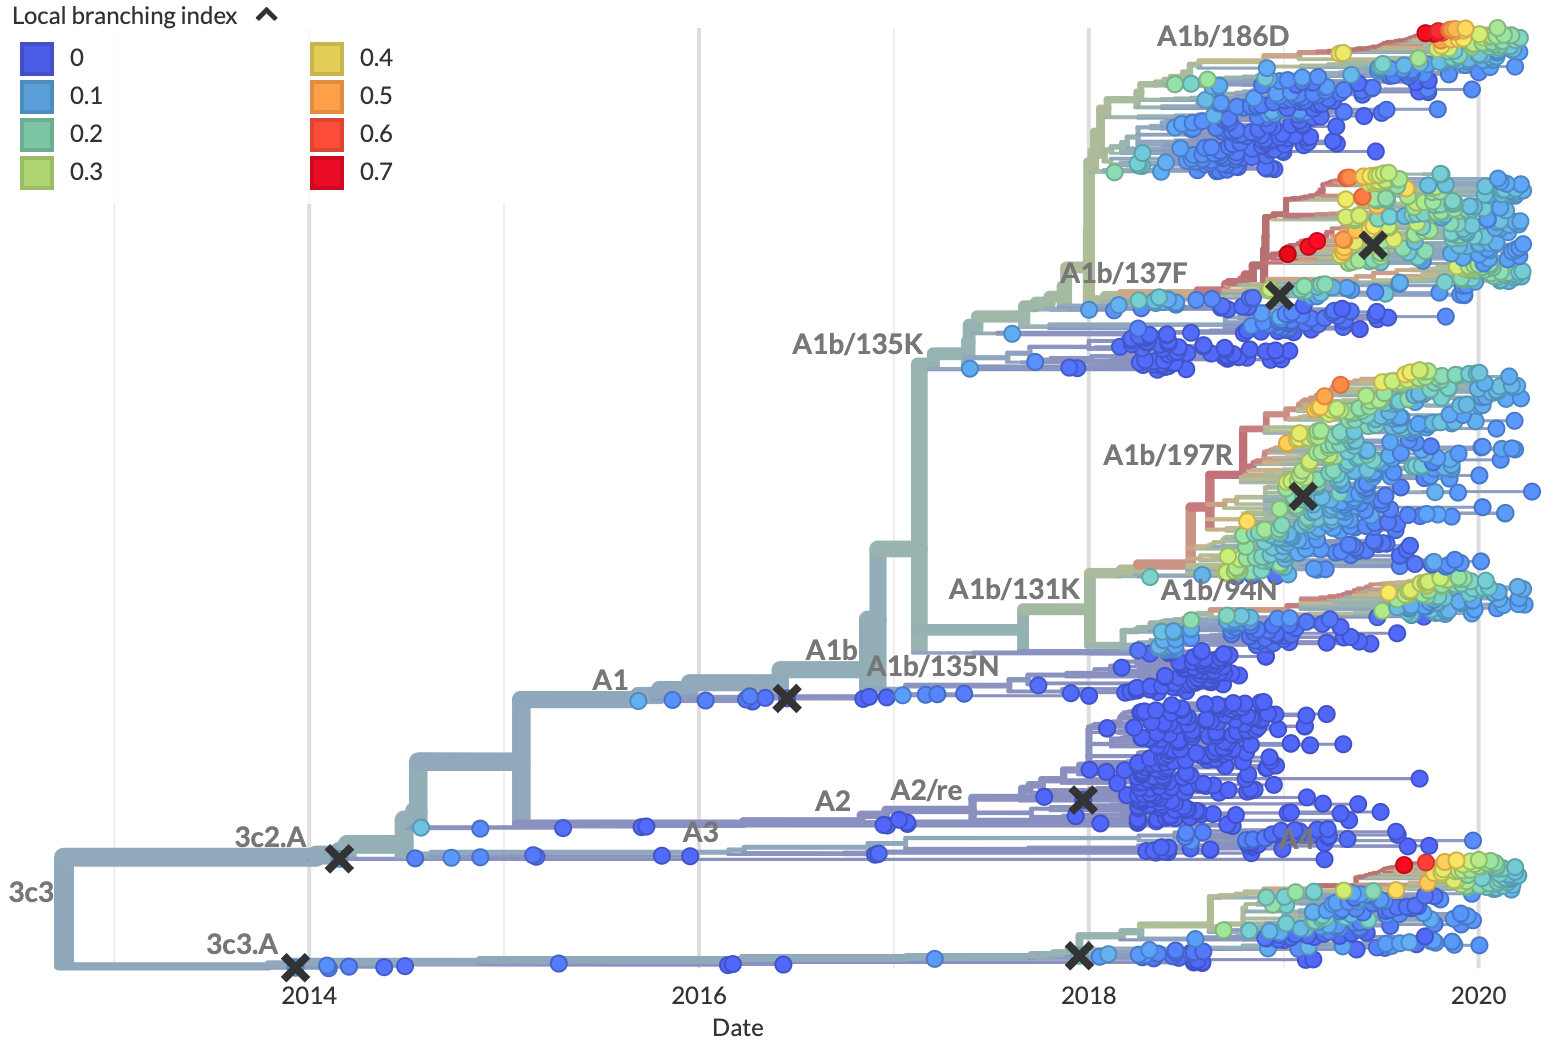
\includegraphics[width=\textwidth]{chapter_05/flu-forecasting-h3n2-lbi-tree.png}
    \label{fig:lbi-practice}
  \end{subfigure}

  \caption{Local branching index (LBI) estimates the fitness of viruses in a phylogeny.
    A) LBI assumes that mutations at the high fitness edge of a current population will seed future populations.
    From Figure 5D of \citet{Neher2013}.
    In practice, LBI tends to identify clusters of recently expanding populations, as shown in this seasonal influenza A/H3N2 phylogeny from Nextstrain.
    \href{https://nextstrain.org/flu/seasonal/h3n2/ha/2y?c=lbi}{Explore LBI values in the current Nextstrain phylogeny for A/H3N2}.
  }
  \label{fig:lbi}
\end{figure}

\citet{Luksza:2014hj} developed a mechanistic model to forecast seasonal influenza evolution based on population genetic theory and previous experimental work.
This model assumed that seasonal influenza viruses grow exponentially as a function of their fitness, compete with each other for hosts through clonal interference, and balance positive effects of mutations at sites previously associated with antigenic drift and deleterious effects of all other mutations.
Instead of predicting the most representative virus of the future population, \citet{Luksza:2014hj} explicitly predicted the future frequencies of entire clades.

Despite the success of these predictive models, other aspects of seasonal influenza evolution complicate predictions.
When multiple beneficial mutations with large effects emerge in a population, the clonal interference between viruses reduces the probability of fixation for all mutations involved.
Seasonal influenza populations also experience multiple bottlenecks in space and time including transmission between hosts, global circulation, and seasonality.
These bottlenecks reduce seasonal influenza's effective population size and reduce the probability that beneficial mutations will sweep globally.
Finally, antigenic escape assays with polyclonal human sera suggest that successful viruses must accumulate multiple beneficial mutations of large effect to successfully evade the diversity of global host immunity \citep{Lee2019}.

\section{How has the field changed since the publication of the first predictive models?}

In the years since the publication of these initial models, significant advances in influenza virology and computational modeling have paved the way for more biologically-informed predictive models.
Recent computational methods can map HI measurements to phylogenetic trees of HA and accurately infer missing measurements between pairs of viruses using their shared ancestry \citep{Neher:2016hy}.
By accounting for variation in viral avidity and serum potency, these methods provide a standardized measurement of antigenic phenotype that can inform existing predictive models.
The application of deep mutational scanning to influenza proteins has enabled high-throughput quantification of functional constraints to protein evolution \citep{Thyagarajan:2014go,Wu:2014ii,Doud:2016gm}.
In addition to these improved measures of HA, recent studies highlight the importance of antigenic effects in neuraminidase (NA) \citep{Chen:2018kp} and fitness effects associated with the reassortment of HA with other proteins \citep{Villa:2017iw}.
The inclusion of evolutionary metrics for the entire influenza genome should therefore improve the predictive power of existing HA-only models.
Finally, a detailed study of influenza phylodynamics has confirmed the importance of global circulation patterns to the success of influenza populations and revealed the variability of these patterns among influenza A and B subtypes \citep{Bedford:2015fj}.
The resulting subtype-specific estimates of migration rate could readily benefit existing predictive models, which currently assume all viruses are panmictic.
Despite the importance of these complementary characteristics of influenza fitness, no current predictive model of influenza evolution integrates all of these phenotypic, genomic, and geographic metrics with existing metrics of antigenic drift from HA sequences.

\section{About this dissertation}

In this dissertation, I describe my independent and collaborative efforts to improve our understanding of seasonal influenza A/H3N2 evolution through novel computational models and data visualizations.
Chapter 2 describes a collaboration with Dr.\ Juhye Lee from the Bloom lab where Juhye performed deep mutational scanning experiments with an A/H3N2 virus and we attempted to understand the relationship between the resulting mutational preferences of A/H3N2 viruses in the lab and the success of mutations in natural populations.
Chapter 3 describes a collaboration with Dr.\ Sarah Hilton from the Bloom lab where we developed a data visualization tool, \emph{dms-view}, that allows virologists to rapidly explore their deep mutational scanning data in the linked contexts of the viral genome and protein structure.
Chapter 3 also describes a preliminary tool for visualization of data from experiments that measure antigenic drift in A/H3N2.
Chapter 4 describes my implementation of a long-term forecasting framework for A/H3N2 populations and how integration of genetic and phenotypic data in this framework produces the most accurate forecasts.
Finally, Chapter 5 synthesizes the findings from the preceding chapters and a recent collaboration with Dr.\ Pierre Barrat-Charlaix from Dr.\ Richard Neher's lab.
This conclusion places the results from this dissertation in the broader context of seasonal influenza evolutionary studies and provides recommendations for future research in the field.
